\chapter{Linear Models for Classification}
\label{ch:classification}

\chapterguide%
  {\chapref{ch:supervised}, \chapref{ch:training}, and probability/odds from \chapref{ch:statistics}.}
  {interpret logistic, softmax, ordinal, and discriminant models; tune thresholds and compare linear classifiers.}

Linear classifiers separate categories with flat boundaries. Logistic regression, discriminant analysis, and the perceptron choose those boundaries differently; QDA extends discriminant analysis to curved boundaries.

\section{Why not just use linear regression?}

OLS on $0/1$ labels can predict outside $[0,1]$. Logistic regression constrains probabilities and fits them with cross-entropy.

\section{From probabilities to odds to a linear model}

\term{Odds} are $p/(1-p)$: $p=0.75$ gives odds~3. Their logarithm, the \term{logit}, spans the real line. Logistic regression assumes linear log-odds:

\begin{mltable}
\begin{tabularx}{0.78\linewidth}{@{}>{\bfseries\leavevmode\color{MLNavy}}X X X@{}}
\toprule
\rowcolor{MLPaleBlue!92}
Probability & Odds & Read aloud \\
\midrule
$50\%$ & $1:1$ & equally likely either way \\
$75\%$ & $3:1$ & three chances for, one against \\
$90\%$ & $9:1$ & nine chances for, one against \\
\bottomrule
\end{tabularx}
\end{mltable}

\[
  \log\frac{p}{1-p}
  =\beta_0+\bm{\beta}^{\mathsf T}\bm{x}.
\]
Solving for $p$ inverts the logarithm and produces the familiar S-shaped \term{sigmoid}:
\[
  P(Y=1\given\bm{x})
  =\sigma(z)
  =\frac{1}{1+e^{-z}},
  \qquad
  z=\beta_0+\bm{\beta}^{\mathsf T}\bm{x}.
\]

\begin{mlfigure}
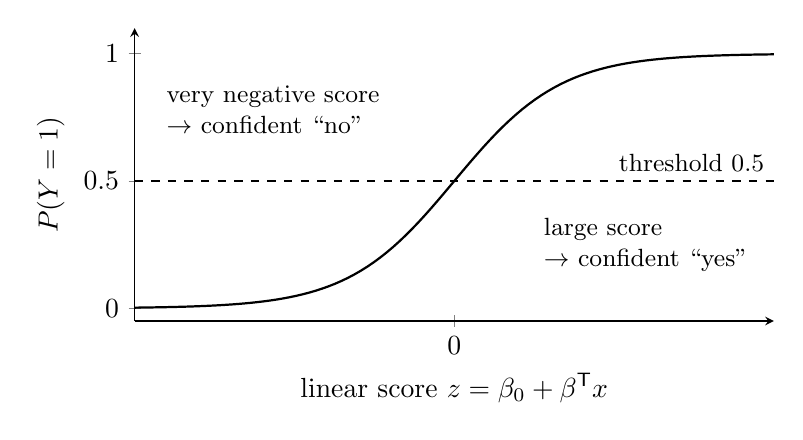
\begin{tikzpicture}
\begin{axis}[
  width=0.80\linewidth, height=5.3cm,
  axis lines=left,
  xlabel={linear score $z=\beta_0+\bm{\beta}^{\mathsf T}\bm{x}$},
  ylabel={$P(Y=1)$},
  ytick={0,0.5,1}, xtick={0},
  domain=-6:6, samples=100, ymin=-0.05, ymax=1.1, clip=false
]
\addplot[thick] {1/(1+exp(-x))};
\draw[dashed] (axis cs:-6,0.5) -- (axis cs:6,0.5)
  node[above left, font=\small] {threshold $0.5$};
\node[font=\small, align=left] at (axis cs:3.6,0.25) {large score\\$\rightarrow$ confident ``yes''};
\node[font=\small, align=left] at (axis cs:-3.4,0.78) {very negative score\\$\rightarrow$ confident ``no''};
\end{axis}
\end{tikzpicture}
\end{mlfigure}

\begin{intuition}
The sigmoid maps an unrestricted score to a probability. Scores near zero give probabilities near $0.5$; large magnitudes indicate confidence.
\end{intuition}

A unit increase in $x_j$ multiplies the odds by $e^{\beta_j}$, holding other features fixed. Thus $\beta_j=0.7$ roughly doubles odds; $-0.7$ roughly halves them.

\begin{workedexample}
Suppose a pass/fail model based on hours studied has $\beta_0=-4$ and $\beta_1=0.08$.
A student with $x=60$ hours has score $z=-4+0.08\times 60=0.8$ and pass probability $\sigma(0.8)\approx 0.69$.
A student with $x=30$ hours has $z=-1.6$ and $\sigma(-1.6)\approx 0.17$.
Each additional hour multiplies the odds of passing by $e^{0.08}\approx 1.083$ --- about an $8\%$ increase in the odds, regardless of the starting point.
\end{workedexample}

\section{Training with cross-entropy}

For binary classification with predicted probability $p$, the loss for one observation is the \term{cross-entropy} (equivalently, the negative log-likelihood of a Bernoulli model from \chapref{ch:statistics}):
\[
  \mathcal{L}(y,p)
  =-[y\log p+(1-y)\log(1-p)].
\]
For $y=1$, loss is $-\log p$, strongly penalizing confident errors. The average-loss gradient is
\[
  \nabla_{\bm{\beta}}J
  =\frac{1}{n}\sum_{i=1}^{n}(p_i-y_i)\,\bm{x}_i,
\]
so updates depend on $p_i-y_i$. Fit iteratively with gradient or Newton-type methods. Convexity rules out nonglobal local minima but does not guarantee a unique finite solution.

\subsection{The decision boundary and the threshold}

At threshold $0.5$, class~1 means $z\ge0$, giving boundary $\beta_0+\bm{\beta}^{\mathsf T}\bm{x}=0$. Tune other thresholds on validation or out-of-fold predictions to reflect error costs (\chapref{ch:evaluation}).

\subsection{Regularization}

Use $L_1$ or $L_2$ penalties with appropriately scaled features and validation-selected strength (\chapref{ch:regression}). Regularization also prevents coefficients diverging on perfectly separable data.

\section{Softmax regression for multiple classes}

For $K$ classes, each class $k$ receives its own weight vector, and the \term{softmax} function converts the $K$ linear scores into probabilities:
\[
  P(Y=k\given\bm{x})
  =\frac{\exp(\bm{\beta}_k^{\mathsf T}\bm{x})}
        {\sum_{j=1}^{K}\exp(\bm{\beta}_j^{\mathsf T}\bm{x})}.
\]
Exponentiating and normalizing preserves score order and makes probabilities sum to one. Training minimizes $\mathcal{L}=-\log P(Y=y\given\bm{x})$.

\term{One-vs-rest} trains $K$ binary classifiers, one class against all others, and predicts the highest-scoring class.

\section{Ordered categories are not ordinary multiclass labels}
\label{sec:ordinal-labels}

\term{Ordinal labels} have order, such as low $<$ medium $<$ high. Softmax ignores order; numerical coding for regression assumes meaningful gaps.

\begin{mltable}
\begin{tabularx}{\linewidth}{@{}p{0.25\linewidth}X@{}}
\toprule
\rowcolor{MLPaleBlue!92}
Approach & When it makes sense \\
\midrule
Ordinary multiclass classifier & Use when categories are genuinely unordered or when order is irrelevant to the decision. \\
Ordinal model / order-aware loss & Prefer when confusing adjacent levels is meaningfully less serious than confusing the two extremes. \\
Regression on integer codes & Use only when the numerical spacing itself is defensible; do not use it merely because the labels can be numbered. \\
\bottomrule
\end{tabularx}
\end{mltable}

Choose order-aware methods or metrics when warranted, and validate whether they help.

\section{Linear discriminant analysis}

Logistic regression is \term{discriminative}: it models $P(y\given\bm{x})$. \term{Linear discriminant analysis (LDA)} is \term{generative}: it models each class's feature distribution and applies Bayes' theorem.

LDA assumes Gaussian classes with means $\bm\mu_k$, shared covariance $\Sigma$, and priors $\pi_k$. Choose the largest discriminant score:
\[
  \delta_k(\bm{x})
  =\bm{x}^{\mathsf T}\Sigma^{-1}\bm{\mu}_k
  -\tfrac{1}{2}\bm{\mu}_k^{\mathsf T}\Sigma^{-1}\bm{\mu}_k
  +\log\pi_k.
\]
Estimate priors from frequencies, means within classes, and covariance from pooled within-class variation. Linear dependence on $\bm x$ gives flat boundaries.

\begin{intuition}
With equal-shaped Gaussian class densities, the tie boundary is linear; class priors shift its position.
\end{intuition}

When to prefer which:

\begin{itemize}
  \item LDA can be stable on small datasets when Gaussian assumptions are reasonable.
  \item Logistic regression assumes less about the features and is more robust when classes are far from Gaussian (heavy tails, strong outliers, many binary features).
  \item LDA also finds up to $K-1$ supervised projection directions for $K$ classes (\chapref{ch:dimred}).
\end{itemize}

\term{Quadratic discriminant analysis (QDA)} drops the shared-covariance assumption and gives each class its own $\Sigma_k$. The boundaries become curved (quadratic), which is more flexible but requires estimating many more parameters --- QDA needs considerably more data per class to stay reliable.

\section{The perceptron}

The \term{perceptron} predicts $\hat y=\operatorname{sign}(\bm w^{\mathsf T}\bm x+b)$ for $y\in\{-1,+1\}$. For each misclassified example, update
\[
  \bm{w}\leftarrow\bm{w}+\eta\,y_i\,\bm{x}_i,
  \qquad
  b\leftarrow b+\eta\,y_i.
\]
Correct predictions cause no update. Separable data yields convergence; otherwise convergence is not guaranteed. The boundary depends on the training path and supplies no probabilities.

\section{Choosing among linear classifiers}

\begin{mltable}
\begin{tabular}{@{}p{0.22\linewidth}p{0.34\linewidth}p{0.34\linewidth}@{}}
\toprule
\rowcolor{MLPaleBlue!92}
Model & Useful strengths & Important limitations \\
\midrule
Logistic regression & Strong probability baseline, convex training, interpretable odds ratios & Linear boundary; probabilities can still be miscalibrated under misspecification or shift \\
LDA & Very fast, stable on small data, gives class-separating directions & Assumes Gaussian classes with shared covariance \\
QDA & Curved boundaries, per-class covariance & Many parameters; needs much more data \\
Perceptron & Simplest possible trainer; historically important & No probabilities; unreliable when classes overlap \\
\bottomrule
\end{tabular}
\end{mltable}

\begin{keyidea}
Logistic regression fits conditional probabilities; LDA models class distributions; the perceptron updates after mistakes. All use flat boundaries, while QDA's separate covariance matrices allow curves.
\end{keyidea}

\begin{modelcard}{Linear Classifiers - Quick Guide}
\begin{tabularx}{\linewidth}{@{}>{\bfseries\leavevmode\color{MLNavy}}p{0.24\linewidth}X@{}}
Best when & A linear boundary is reasonable, fast prediction matters, or coefficients need to be interpreted. \cr
Start with & Logistic regression for probabilities; softmax regression for several classes. \cr
Preprocessing & Encode categories, standardize numerical features for regularization, and handle imbalance with suitable metrics or weights. \cr
Main controls & Regularization strength, penalty type, and the probability threshold used for decisions. \cr
Watch for & Nonlinear class structure, poorly calibrated probabilities, rare classes, and causal over-interpretation (\secref{sec:correlation}). \cr
\end{tabularx}
\end{modelcard}

\section{Using linear classifiers in practice}
\label{sec:logistic-practice}

\subsection{Moving the threshold on purpose}

One fitted model, three thresholds. These are the Titanic validation results printed in Lab~2, Part~C:

\begin{mltable}
\begin{tabularx}{0.82\linewidth}{@{}>{\bfseries\leavevmode\color{MLNavy}}p{0.2\linewidth}X X X@{}}
\toprule
\rowcolor{MLPaleBlue!92}
Threshold & Precision & Recall & What changed \\
\midrule
$0.30$ & $0.64$ & $0.81$ & many passengers flagged; most survivors caught \\
$0.50$ & $0.73$ & $0.67$ & the default \\
$0.70$ & $0.90$ & $0.50$ & few flagged; half the survivors missed \\
\bottomrule
\end{tabularx}
\end{mltable}

\begin{intuition}
Only the cutoff changes. Lower thresholds favor recall; higher thresholds reduce alerts. Choose using costs and response capacity.
\end{intuition}

Choose the operating point from out-of-fold predictions and a stated cost or capacity constraint. Then refit the model on all training data and assess that locked rule on the test set once.

\subsection{Reading the coefficients}

\begin{workedexample}
For an ``hours studied'' coefficient of $0.62$, each extra hour multiplies passing odds by $e^{0.62}\approx1.86$, holding other features fixed. The probability increase depends on the starting probability.
\end{workedexample}

\subsection{More than two classes}

\begin{mlfigure}
\begin{tikzpicture}[
  node distance=0.36cm and 0.62cm,
  sc/.style={draw=MLBlue,fill=MLPaleBlue,rounded corners=1.2mm,minimum width=1.55cm,minimum height=0.6cm,align=center,font=\scriptsize\color{MLNavy}},
  pr/.style={draw=MLGreen,fill=MLPaleTeal,rounded corners=1.2mm,minimum width=1.55cm,minimum height=0.6cm,align=center,font=\scriptsize\color{MLNavy}},
  arr/.style={-{Stealth[length=2mm]},thick,draw=MLTeal}
]
\node[sc] (s1) {cat: $1.2$};
\node[sc,below=of s1] (s2) {dog: $3.4$};
\node[sc,below=of s2] (s3) {fox: $2.0$};
\node[draw=MLOrange,fill=MLPaleOrange,rounded corners=2mm,minimum height=2.5cm,minimum width=1.9cm,align=center,font=\scriptsize\bfseries\color{MLNavy},right=1.0cm of s2] (sm) {softmax\\[0.15em]\scriptsize\mdseries exponentiate,\\then divide by\\the total};
\node[pr,right=1.0cm of sm] (p2) {dog: $0.75$};
\node[pr,above=of p2] (p1) {cat: $0.08$};
\node[pr,below=of p2] (p3) {fox: $0.17$};
\draw[arr] (s1.east) -- (sm.west); \draw[arr] (s2.east) -- (sm.west); \draw[arr] (s3.east) -- (sm.west);
\draw[arr] (sm.east) -- (p1.west); \draw[arr] (sm.east) -- (p2.west); \draw[arr] (sm.east) -- (p3.west);
\node[font=\scriptsize\itshape\color{MLMuted},below=0.3cm of p3] {always adds to 1.00};
\end{tikzpicture}
\end{mlfigure}

\begin{keyidea}
Softmax preserves score order while normalizing exponentials to a probability distribution.
\end{keyidea}

\begin{tryit}
Fit logistic regression and obtain out-of-fold training probabilities. Sweep thresholds from 0.05 to 0.95 in steps of 0.05; plot precision against recall without using test data.
\end{tryit}

\begin{debugtask}
A teammate lowers the probability threshold until test-set recall reaches the desired value, then reports that same test recall as final performance. Explain the leakage in model selection and show where threshold tuning belongs instead.
\end{debugtask}

\begin{decisionmemo}
For a rare positive class, choose between an unweighted logistic model, class weighting, and a lower decision threshold. State which quantity each intervention changes, which validation metric you would inspect, and why the three options are not interchangeable.
\end{decisionmemo}

\labsection{2}{Supervised learning I: regression, classification, and the workflow}{sec:lab02-supervised-workflow}

\begin{labproject}{Two regression examples, two classification examples, and a saved model at the end}
\textbf{Goal.} Fit regression/classification pipelines, validate chronologically where needed, tune thresholds and hyperparameters, test once, and save models.

\medskip\noindent\textbf{Setup.}\par
\begin{lstlisting}[style=mlpython]
import json
from pathlib import Path

import joblib
import matplotlib.pyplot as plt
import numpy as np
import pandas as pd
import sklearn
from sklearn.compose import ColumnTransformer
from sklearn.ensemble import RandomForestClassifier, RandomForestRegressor
from sklearn.impute import SimpleImputer
from sklearn.linear_model import LinearRegression, LogisticRegression, Ridge
from sklearn.metrics import (
    ConfusionMatrixDisplay,
    PrecisionRecallDisplay,
    RocCurveDisplay,
    accuracy_score,
    average_precision_score,
    classification_report,
    confusion_matrix,
    mean_absolute_error,
    mean_squared_error,
    precision_score,
    r2_score,
    recall_score,
    roc_auc_score,
)
from sklearn.model_selection import GridSearchCV, StratifiedKFold, train_test_split
from sklearn.pipeline import Pipeline
from sklearn.preprocessing import OneHotEncoder, StandardScaler

PROJECT_ROOT = Path.cwd().parent
DATA = PROJECT_ROOT / "all_datasets"
MODELS = PROJECT_ROOT / "models"
MODELS.mkdir(exist_ok=True)
\end{lstlisting}

Use one helper for numerical imputation/scaling and categorical imputation/one-hot encoding.

\begin{lstlisting}[style=mlpython]
def make_preprocess(num_cols, cat_cols):
    return ColumnTransformer([
        ("num", Pipeline([
            ("impute", SimpleImputer(strategy="median")),
            ("scale", StandardScaler()),
        ]), num_cols),
        ("cat", Pipeline([
            ("impute", SimpleImputer(strategy="most_frequent")),
            ("onehot", OneHotEncoder(handle_unknown="ignore")),
        ]), cat_cols),
    ])
\end{lstlisting}

\medskip\noindent\textbf{Part A --- Regression: ordinary least squares versus ridge.}\par

Predict insurance \texttt{charges}. Compare OLS and ridge on the same features and split.

\begin{lstlisting}[style=mlpython]
insurance = pd.read_csv(DATA / "medical_cost_personal_dataset.csv")
print(insurance.head())

X = insurance.drop(columns="charges")
y = insurance["charges"]
num_cols = ["age", "bmi", "children"]
cat_cols = ["sex", "smoker", "region"]

X_train, X_valid, y_train, y_valid = train_test_split(
    X, y, test_size=0.20, random_state=42
)
\end{lstlisting}

MAE gives average dollar error; RMSE emphasizes extremes; $R^2$ compares squared error with the mean-label reference.

\begin{lstlisting}[style=mlpython]
fitted = {}
predictions = {}

for name, estimator in {
    "linear regression": LinearRegression(),
    "ridge": Ridge(alpha=10.0),
}.items():
    model = Pipeline([("preprocess", make_preprocess(num_cols, cat_cols)), ("model", estimator)])
    model.fit(X_train, y_train)
    fitted[name] = model
    predictions[name] = model.predict(X_valid)
    pred = predictions[name]
    print(f"\n{name}")
    print("MAE:", round(mean_absolute_error(y_valid, pred), 2))
    print("RMSE:", round(np.sqrt(mean_squared_error(y_valid, pred)), 2))
    print("R2:", round(r2_score(y_valid, pred), 3))
\end{lstlisting}

Coefficients give conditional prediction changes. Standardized numerical coefficients represent one-standard-deviation changes.

\begin{lstlisting}[style=mlpython]
linear = fitted["linear regression"]
names = linear.named_steps["preprocess"].get_feature_names_out()
coefs = pd.Series(linear.named_steps["model"].coef_, index=names).sort_values()

plt.figure(figsize=(6, 3.6))
plt.barh(coefs.index, coefs.values)
plt.axvline(0, color="grey", linewidth=0.8)
plt.xlabel("Change in predicted charges (dollars)")
plt.title("What the linear model learned")
plt.tight_layout()
plt.show()
\end{lstlisting}

\textbf{Inspect.} The smoker coefficient exceeds \$20,000; age and BMI contribute more than region. These are model associations, not causal effects.

Plot ridge residuals; structure suggests missed patterns.

\begin{lstlisting}[style=mlpython]
ridge_pred = predictions["ridge"]
residual = y_valid.to_numpy() - ridge_pred
is_smoker = (X_valid["smoker"] == "yes").to_numpy()

fig, axes = plt.subplots(1, 2, figsize=(9.5, 3.8))
axes[0].scatter(y_valid[~is_smoker], ridge_pred[~is_smoker], alpha=0.5, label="non-smoker")
axes[0].scatter(y_valid[is_smoker], ridge_pred[is_smoker], alpha=0.5, label="smoker")
axes[0].plot([0, y_valid.max()], [0, y_valid.max()], linestyle="--", color="grey")
axes[0].set_xlabel("Actual charges")
axes[0].set_ylabel("Predicted charges")
axes[0].set_title("Ridge: actual versus predicted")
axes[0].legend()
axes[1].scatter(ridge_pred, residual, alpha=0.6)
axes[1].axhline(0, linestyle="--", color="grey")
axes[1].set_xlabel("Predicted charges")
axes[1].set_ylabel("Residual (actual - predicted)")
axes[1].set_title("Ridge: residual plot")
plt.tight_layout()
plt.show()
\end{lstlisting}

\textbf{Inspect.} Smoker bands suggest a smoker $\times$ BMI interaction. Shrinkage alone cannot add this missing structure.

\medskip\noindent\textbf{Part B --- Regression on a time series: validate in date order.}\par

Sort two years of daily rentals by date; reserve the last 20\% for validation to avoid training on future days.

\begin{lstlisting}[style=mlpython]
bikes = pd.read_csv(DATA / "bike_sharing_dataset_day.csv")
bikes["dteday"] = pd.to_datetime(bikes["dteday"])
bikes = bikes.sort_values("dteday").reset_index(drop=True)

# cnt = casual + registered, so those two columns would leak the answer.
bike_cat = ["season", "yr", "mnth", "holiday", "weekday", "workingday", "weathersit"]
bike_num = ["temp", "atemp", "hum", "windspeed"]
X_b = bikes[bike_cat + bike_num]
y_b = bikes["cnt"]

cut = int(len(bikes) * 0.80)
print("train:", bikes["dteday"].iloc[0].date(), "to", bikes["dteday"].iloc[cut - 1].date())
print("valid:", bikes["dteday"].iloc[cut].date(), "to", bikes["dteday"].iloc[-1].date())
\end{lstlisting}

One-hot encode calendar categories; pass numerical weather features directly to the unscaled tree model.

\begin{lstlisting}[style=mlpython]
Xb_train, Xb_valid = X_b.iloc[:cut], X_b.iloc[cut:]
yb_train, yb_valid = y_b.iloc[:cut], y_b.iloc[cut:]
dates_valid = bikes["dteday"].iloc[cut:]

bike_model = Pipeline([
    ("preprocess", ColumnTransformer([
        ("cat", OneHotEncoder(handle_unknown="ignore"), bike_cat),
        ("num", "passthrough", bike_num),
    ])),
    ("model", RandomForestRegressor(
        n_estimators=400, min_samples_leaf=2, random_state=42, n_jobs=-1
    )),
])
bike_model.fit(Xb_train, yb_train)
bike_pred = bike_model.predict(Xb_valid)
print("daily MAE:", round(mean_absolute_error(yb_valid, bike_pred), 1),
      " (mean daily demand in validation:", round(yb_valid.mean(), 1), ")")

plt.figure(figsize=(8, 3.6))
plt.plot(dates_valid, yb_valid.to_numpy(), label="actual")
plt.plot(dates_valid, bike_pred, label="predicted")
plt.xlabel("Date")
plt.ylabel("Daily rentals")
plt.title("Chronological validation: actual versus predicted demand")
plt.legend()
plt.tight_layout()
plt.show()
\end{lstlisting}

\textbf{Inspect.} The forest tracks seasonality but underpredicts peaks beyond the training-label range; it cannot extrapolate.

Repeat chronologically on 17,379 hourly rows, adding \texttt{hr}; plot one validation week.

\begin{lstlisting}[style=mlpython]
hourly = pd.read_csv(DATA / "bike_sharing_dataset_hour.csv")
hourly["dteday"] = pd.to_datetime(hourly["dteday"])
hourly = hourly.sort_values(["dteday", "hr"]).reset_index(drop=True)

hour_cat = bike_cat + ["hr"]
Xh = hourly[hour_cat + bike_num]
yh = hourly["cnt"]
cut_h = int(len(hourly) * 0.80)

hour_model = Pipeline([
    ("preprocess", ColumnTransformer([
        ("cat", OneHotEncoder(handle_unknown="ignore"), hour_cat),
        ("num", "passthrough", bike_num),
    ])),
    ("model", RandomForestRegressor(
        n_estimators=200, min_samples_leaf=2, random_state=42, n_jobs=-1
    )),
])
hour_model.fit(Xh.iloc[:cut_h], yh.iloc[:cut_h])
hour_pred = hour_model.predict(Xh.iloc[cut_h:])
print("hourly MAE:", round(mean_absolute_error(yh.iloc[cut_h:], hour_pred), 1),
      " (mean hourly demand in validation:", round(yh.iloc[cut_h:].mean(), 1), ")")

week = slice(0, 24 * 7)
plt.figure(figsize=(9, 3.4))
plt.plot(range(24 * 7), yh.iloc[cut_h:].to_numpy()[week], label="actual")
plt.plot(range(24 * 7), hour_pred[week], label="predicted")
plt.xlabel("Hour of the first validation week")
plt.ylabel("Rentals per hour")
plt.title("Hourly demand has a shape that hr captures")
plt.legend()
plt.tight_layout()
plt.show()
\end{lstlisting}

\textbf{Inspect.} Working days have two peaks; weekends one. Lab~8 predicts this series from 24 previous hours.

\medskip\noindent\textbf{Part C --- Classification: baselines, probabilities, and the threshold.}\par

Compare logistic regression and a forest using seven passenger features, no identifiers, and stratified splits. Accuracy evaluates thresholded decisions; AUC evaluates ranking.

\begin{lstlisting}[style=mlpython]
titanic = pd.read_csv(DATA / "titanic_dataset.csv")

features = ["Pclass", "Sex", "Age", "SibSp", "Parch", "Fare", "Embarked"]
t_num = ["Age", "SibSp", "Parch", "Fare"]
t_cat = ["Pclass", "Sex", "Embarked"]
X_t = titanic[features]
y_t = titanic["Survived"]

Xt_train, Xt_valid, yt_train, yt_valid = train_test_split(
    X_t, y_t, test_size=0.25, random_state=42, stratify=y_t
)
print("majority-class baseline accuracy:", round(1 - yt_valid.mean(), 3))

scores = {}
fitted_t = {}
for name, estimator in {
    "logistic": LogisticRegression(max_iter=1000),
    "random_forest": RandomForestClassifier(n_estimators=300, min_samples_leaf=2,
                                            random_state=42),
}.items():
    pipe = Pipeline([("preprocess", make_preprocess(t_num, t_cat)), ("model", estimator)])
    pipe.fit(Xt_train, yt_train)
    fitted_t[name] = pipe
    scores[name] = {"accuracy": accuracy_score(yt_valid, pipe.predict(Xt_valid)),
                    "roc_auc": roc_auc_score(yt_valid, pipe.predict_proba(Xt_valid)[:, 1])}
    print(f"{name:14s} accuracy={scores[name]['accuracy']:.3f} "
          f"roc_auc={scores[name]['roc_auc']:.3f}")

# The same logistic model, three decision rules (the table in the notes).
prob_t = fitted_t["logistic"].predict_proba(Xt_valid)[:, 1]
for threshold in [0.30, 0.50, 0.70]:
    pred_t = (prob_t >= threshold).astype(int)
    print(f"threshold {threshold:.2f}: precision={precision_score(yt_valid, pred_t):.2f} "
          f"recall={recall_score(yt_valid, pred_t):.2f}")

pd.DataFrame(scores).T.plot.bar(figsize=(5, 3.2), ylim=(0.5, 1.0), rot=0)
plt.axhline(1 - yt_valid.mean(), linestyle="--", color="grey", label="majority baseline")
plt.title("Two models, two metrics, one validation split")
plt.legend(loc="lower right")
plt.tight_layout()
plt.show()
\end{lstlisting}

\textbf{Inspect.} Both beat the baseline, but metric rankings differ. Use Part~D cross-validation to assess small differences.

For 30 tumor measurements, predict \texttt{M} versus \texttt{B}. Plot probabilities by true class; a threshold marks malignant decisions.

\begin{lstlisting}[style=mlpython]
cancer = pd.read_csv(DATA / "breast_cancer_dataset.csv")

X_c = cancer.drop(columns=["id", "diagnosis", "Unnamed: 32"], errors="ignore")
y_c = (cancer["diagnosis"] == "M").astype(int)

Xc_train, Xc_valid, yc_train, yc_valid = train_test_split(
    X_c, y_c, test_size=0.25, random_state=42, stratify=y_c
)

cancer_model = Pipeline([
    ("scale", StandardScaler()),
    ("model", LogisticRegression(max_iter=2000)),
])
cancer_model.fit(Xc_train, yc_train)
prob = cancer_model.predict_proba(Xc_valid)[:, 1]

plt.figure(figsize=(6, 3.4))
plt.hist(prob[yc_valid == 0], bins=25, alpha=0.6, label="benign (actual)")
plt.hist(prob[yc_valid == 1], bins=25, alpha=0.6, label="malignant (actual)")
plt.axvline(0.50, color="black", linestyle="--", label="threshold 0.50")
plt.axvline(0.30, color="red", linestyle=":", label="threshold 0.30")
plt.xlabel("Predicted probability of malignant")
plt.ylabel("Tumours")
plt.title("A threshold is a vertical line through this picture")
plt.legend()
plt.tight_layout()
plt.show()
\end{lstlisting}

Confusion-matrix rows are truth; columns are decisions. Precision measures correct malignant alerts; recall measures detected malignancies. Lowering the threshold increases alerts and cannot reduce recall.

\begin{lstlisting}[style=mlpython]
for threshold in [0.50, 0.30]:
    pred = (prob >= threshold).astype(int)
    print(f"\nthreshold = {threshold:.2f}")
    print(confusion_matrix(yc_valid, pred))
    print(classification_report(yc_valid, pred, digits=3))
    ConfusionMatrixDisplay.from_predictions(yc_valid, pred, display_labels=["benign", "malignant"])
    plt.title(f"Confusion matrix at threshold {threshold:.2f}")
    plt.tight_layout()
    plt.show()

thresholds = np.linspace(0.05, 0.95, 19)
precisions = [precision_score(yc_valid, (prob >= t).astype(int), zero_division=0)
              for t in thresholds]
recalls = [recall_score(yc_valid, (prob >= t).astype(int)) for t in thresholds]

plt.figure(figsize=(6, 3.4))
plt.plot(thresholds, precisions, marker="o", label="precision")
plt.plot(thresholds, recalls, marker="o", label="recall")
plt.xlabel("Decision threshold")
plt.ylabel("Score")
plt.title("The threshold trades recall for precision")
plt.legend()
plt.tight_layout()
plt.show()
\end{lstlisting}

ROC AUC measures ranking across classes; average precision summarizes precision--recall, emphasizing positive retrieval.

\begin{lstlisting}[style=mlpython]
print("ROC AUC:", round(roc_auc_score(yc_valid, prob), 3))
print("PR AUC:", round(average_precision_score(yc_valid, prob), 3))

fig, axes = plt.subplots(1, 2, figsize=(9, 3.6))
RocCurveDisplay.from_predictions(yc_valid, prob, ax=axes[0])
axes[0].set_title("ROC curve")
PrecisionRecallDisplay.from_predictions(yc_valid, prob, ax=axes[1])
axes[1].set_title("Precision-recall curve")
plt.tight_layout()
plt.show()
\end{lstlisting}

\medskip\noindent\textbf{Part D --- Tune with cross-validation, then test once.}\par

Reserve Titanic test rows. Within training data, use five-fold CV to tune \texttt{C} and \texttt{class\_weight}; refit the winner on all training rows.

\begin{lstlisting}[style=mlpython]
X_train, X_test, y_train, y_test = train_test_split(
    X_t, y_t, test_size=0.25, random_state=42, stratify=y_t
)

search = GridSearchCV(
    Pipeline([("preprocess", make_preprocess(t_num, t_cat)),
              ("model", LogisticRegression(max_iter=2000))]),
    param_grid={
        "model__C": [0.01, 0.1, 1.0, 10.0, 100.0],
        "model__class_weight": [None, "balanced"],
    },
    scoring="roc_auc",
    cv=StratifiedKFold(n_splits=5, shuffle=True, random_state=42),
    n_jobs=-1,
)
search.fit(X_train, y_train)

cv_table = pd.DataFrame(search.cv_results_)
plt.figure(figsize=(5.5, 3.4))
for weight, group in cv_table.groupby(cv_table["param_model__class_weight"].astype(str)):
    plt.errorbar(group["param_model__C"].astype(float), group["mean_test_score"],
                 yerr=group["std_test_score"], marker="o", capsize=3, label=f"class_weight={weight}")
plt.xscale("log")
plt.xlabel("C (weaker regularization to the right)")
plt.ylabel("Cross-validated ROC AUC")
plt.title("What the grid search saw")
plt.legend()
plt.tight_layout()
plt.show()
\end{lstlisting}

\textbf{Inspect.} Fold spread exceeds many differences between settings; avoid overinterpreting small gains.

Only now is the test set touched, once.

\begin{lstlisting}[style=mlpython]
test_prob = search.predict_proba(X_test)[:, 1]
test_auc = roc_auc_score(y_test, test_prob)

print("best parameters:", search.best_params_)
print("cross-validated ROC AUC:", round(search.best_score_, 3))
print("final test ROC AUC:", round(test_auc, 3))
\end{lstlisting}

\medskip\noindent\textbf{Part E --- Save the models and use them.}\par

Save preprocessing and estimator together with \texttt{joblib.dump}; add a card documenting inputs and evaluation.

\begin{lstlisting}[style=mlpython]
final_model = search.best_estimator_
model_path = MODELS / "titanic_survival.joblib"
joblib.dump(final_model, model_path)

card = {
    "task": "predict Titanic survival (1 = survived)",
    "features": features,
    "model": "logistic regression pipeline",
    "best_parameters": search.best_params_,
    "training_rows": int(len(X_train)),
    "final_test_roc_auc": round(float(test_auc), 3),
    "decision_threshold": 0.5,
    "scikit_learn_version": sklearn.__version__,
}
(MODELS / "titanic_survival_card.json").write_text(json.dumps(card, indent=2))
size_kb = model_path.stat().st_size / 1024
print(f"saved: {model_path.name} ({size_kb:.1f} KB) and titanic_survival_card.json")
\end{lstlisting}

Load the pipeline and predict new rows with matching columns, without retraining. Repeat for insurance customers differing in one feature.

\begin{lstlisting}[style=mlpython]
loaded = joblib.load(model_path)
new_passengers = pd.DataFrame([
    {"Pclass": 1, "Sex": "female", "Age": 29, "SibSp": 0, "Parch": 0, "Fare": 80.0, "Embarked": "C"},
    {"Pclass": 3, "Sex": "male",   "Age": 40, "SibSp": 0, "Parch": 0, "Fare":  7.9, "Embarked": "S"},
])
new_passengers["survival_probability"] = loaded.predict_proba(new_passengers)[:, 1].round(3)
print(new_passengers)

joblib.dump(fitted["linear regression"], MODELS / "insurance_charges.joblib")
pricing = joblib.load(MODELS / "insurance_charges.joblib")
new_customer = pd.DataFrame([
    {"age": 35, "sex": "female", "bmi": 27.5, "children": 2, "smoker": "no", "region": "southeast"},
    {"age": 35, "sex": "female", "bmi": 27.5, "children": 2, "smoker": "yes", "region": "southeast"},
])
new_customer["predicted_charges"] = pricing.predict(new_customer).round(0)
print(new_customer)
\end{lstlisting}

Run the saved passenger model from the terminal:

\begin{lstlisting}[style=mlterminal]
python predict_passenger.py --pclass 2 --sex female --age 30 --fare 20
\end{lstlisting}

\begin{tryit}
Run the Part~C classification workflow on \texttt{heart\_failure\_dataset.csv} (label \texttt{HeartDisease}). Build the column lists from the data types with \texttt{select\_dtypes}, reuse \texttt{make\_preprocess}, and report accuracy, ROC AUC, and the confusion matrix at threshold 0.5.
\end{tryit}

\begin{decisionmemo}
Choose a threshold when missed positives cost more than false alarms. Explain confusion-matrix changes and justify the choice using Part C validation evidence.
\end{decisionmemo}
\end{labproject}


\begin{quickcheck}
\begin{enumerate}
  \item Why is logistic regression called a linear classifier even though it outputs a nonlinear sigmoid probability?
  \item Why should the probability model and the operational classification threshold be treated as separate objects?
  \item What changes when binary logistic regression is extended to a multiclass softmax model?
\end{enumerate}
\end{quickcheck}
